\documentclass{article}
\usepackage[utf8]{inputenc}
\usepackage[top=1.25in, bottom=1.25in, left=1.5in, right=1.5in]{geometry}
\usepackage{graphicx}

\title{\vspace{5cm}\textbf{Mesa Interactiva BarISTa}\\Manual de Utilizador}

\begin{document}
\maketitle
\newpage

\tableofcontents
\newpage

\section{A aplicação BarISTa}
\section{Pedidos}
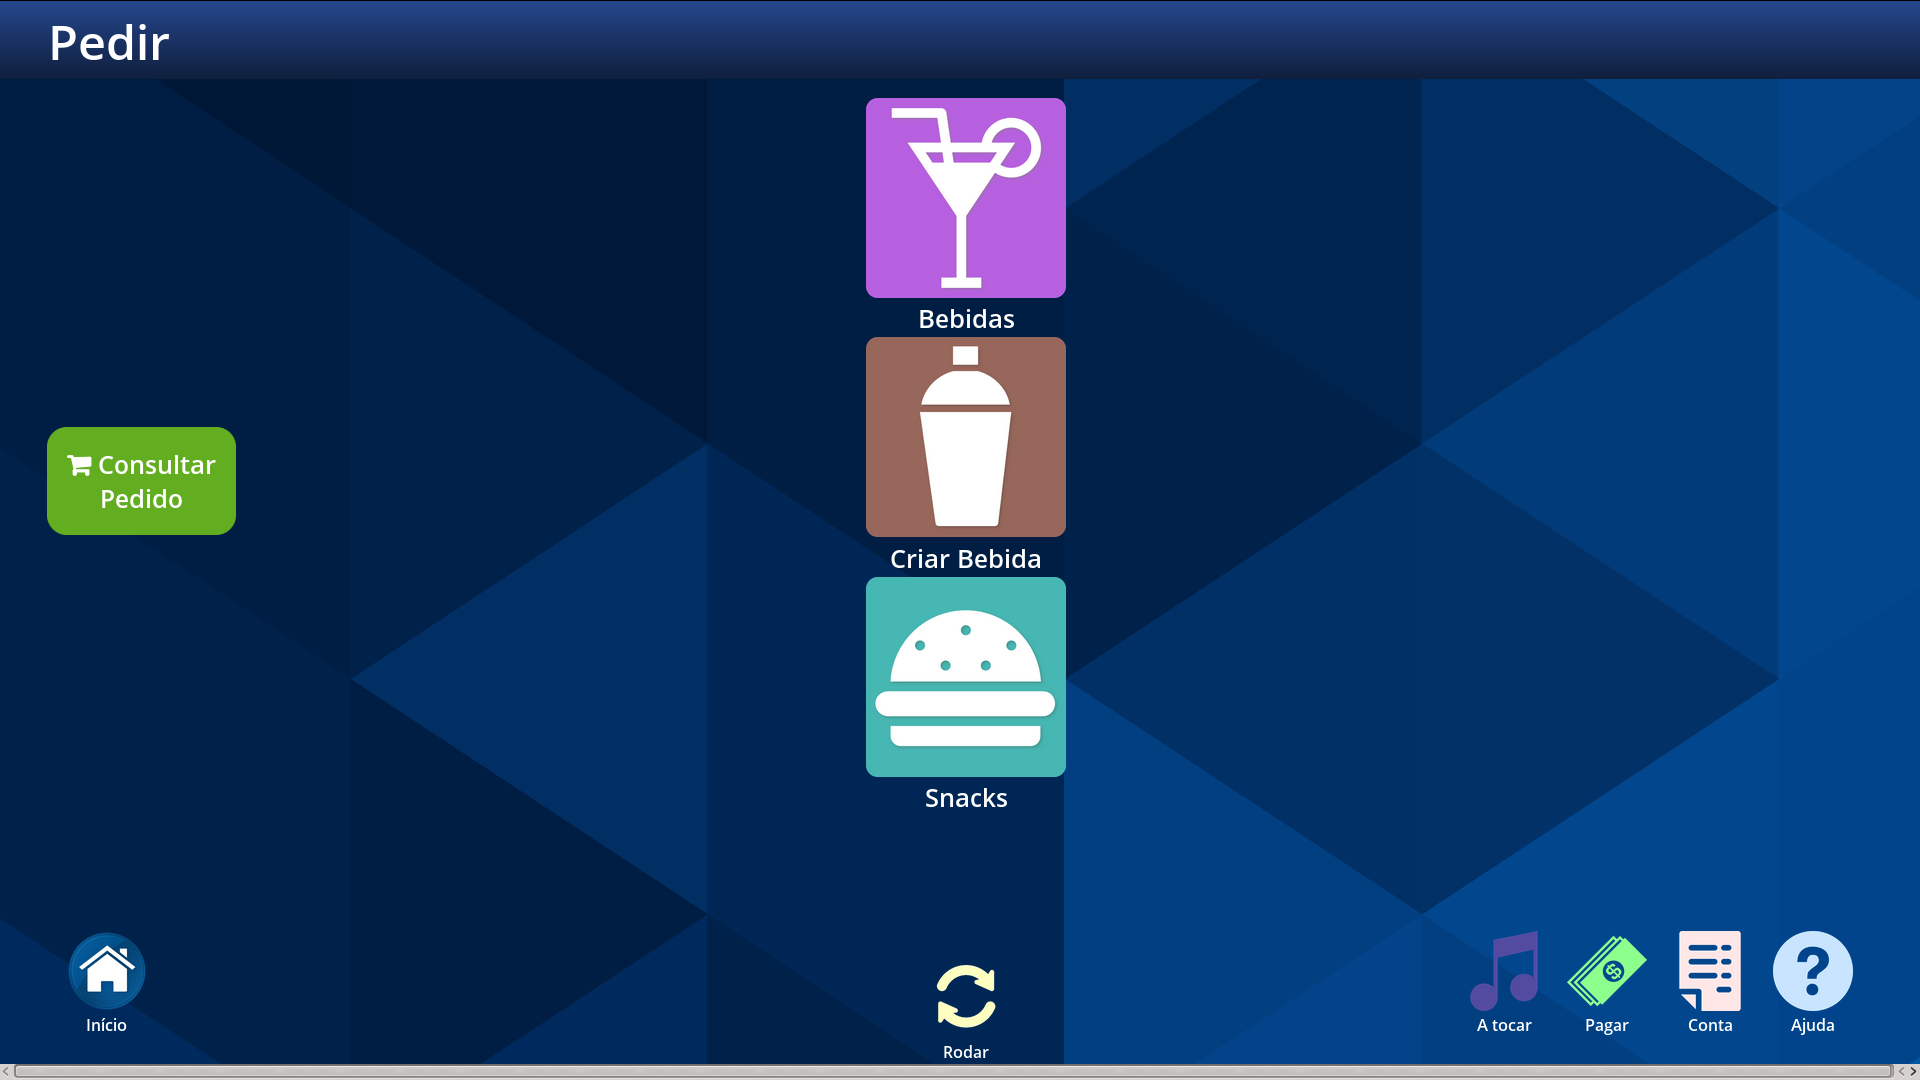
\includegraphics[width=15cm, height=8cm]{user_manual_images/order_menu.png}
\subsection{Pedir uma bebida ou snack}
Para pedir uma bebida ou um snack neste menu, o utilizador têm de pressionar o botão que lhe corresponde, sendo que aparece um menu lateral onde este pode adicionar bebidas ao carrinho.\\
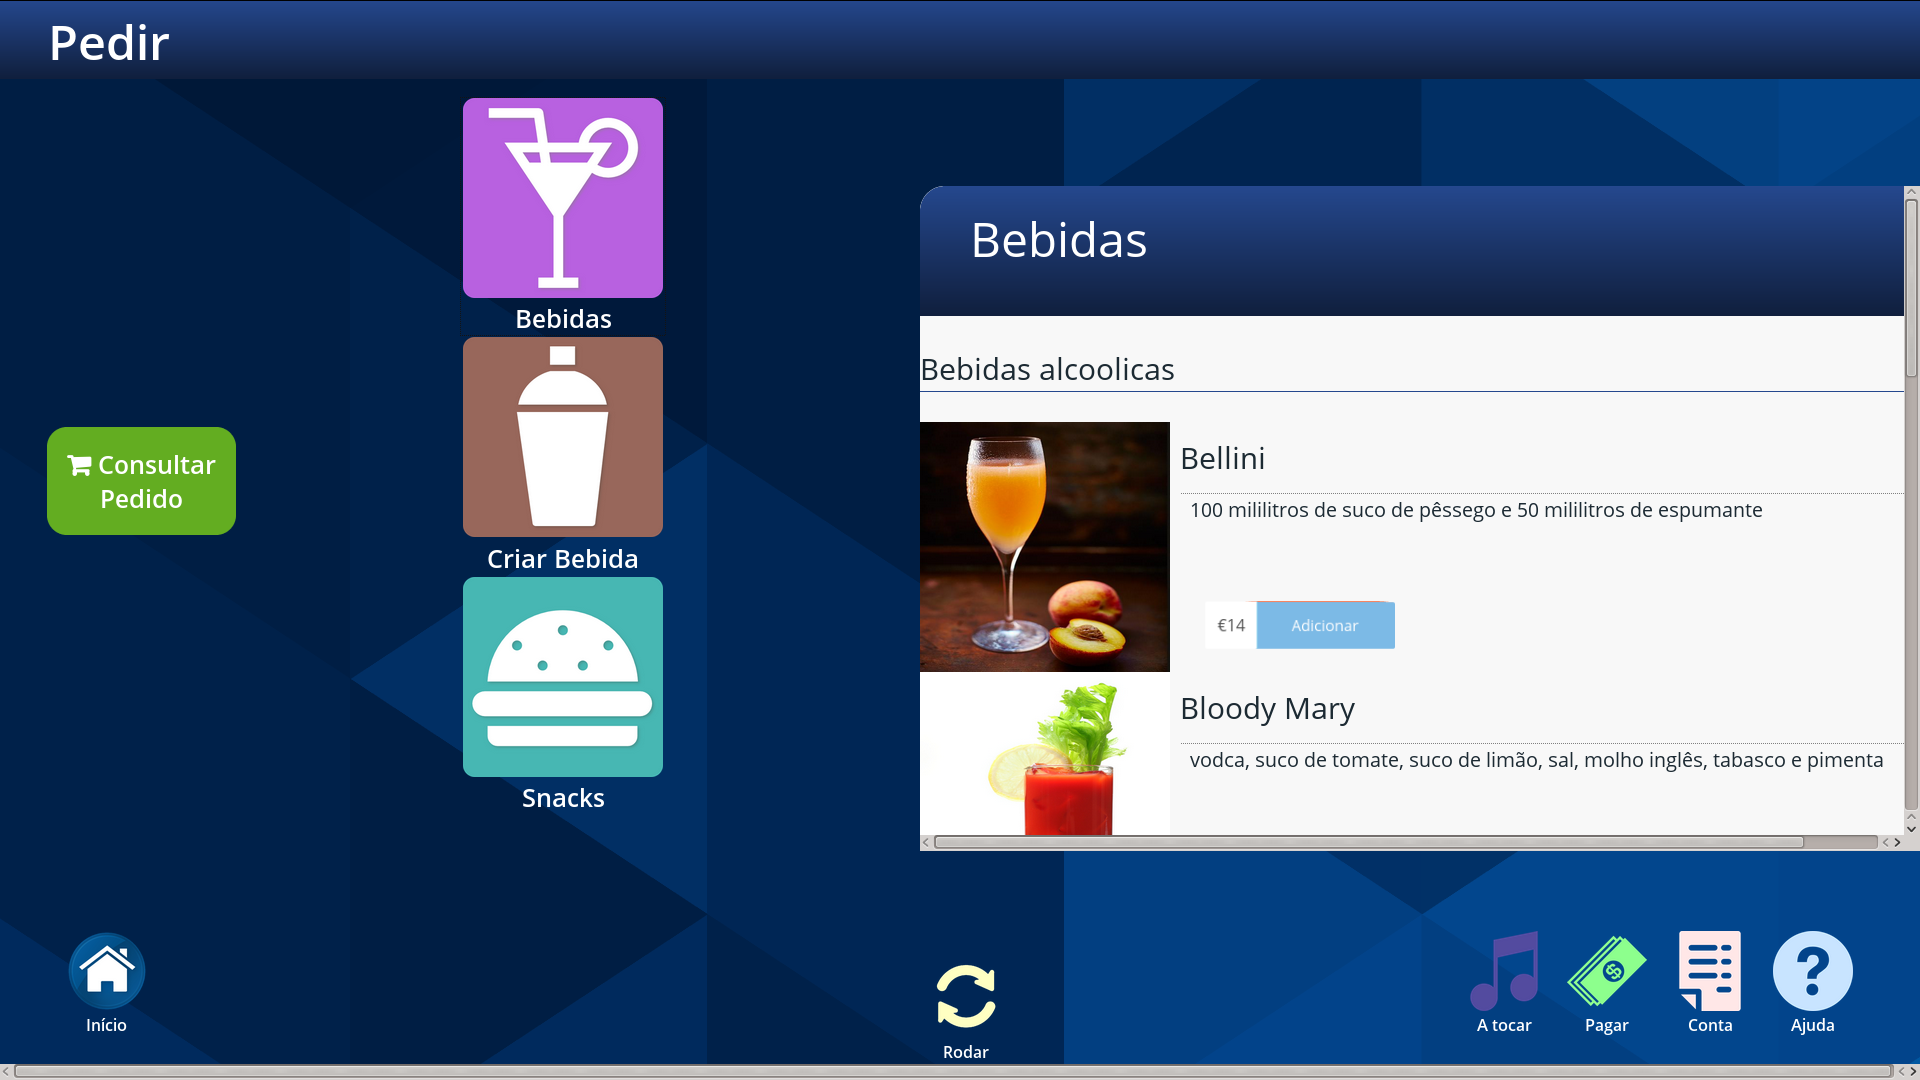
\includegraphics[width=15cm, height=8cm]{user_manual_images/drinks_submenu.png} Após ter escolhido as bebidas/snacks, para confirmar o pedido, o utilizador tem de pressionar o botão Consultar Pedido, e de seguida o botão Pedir.\\
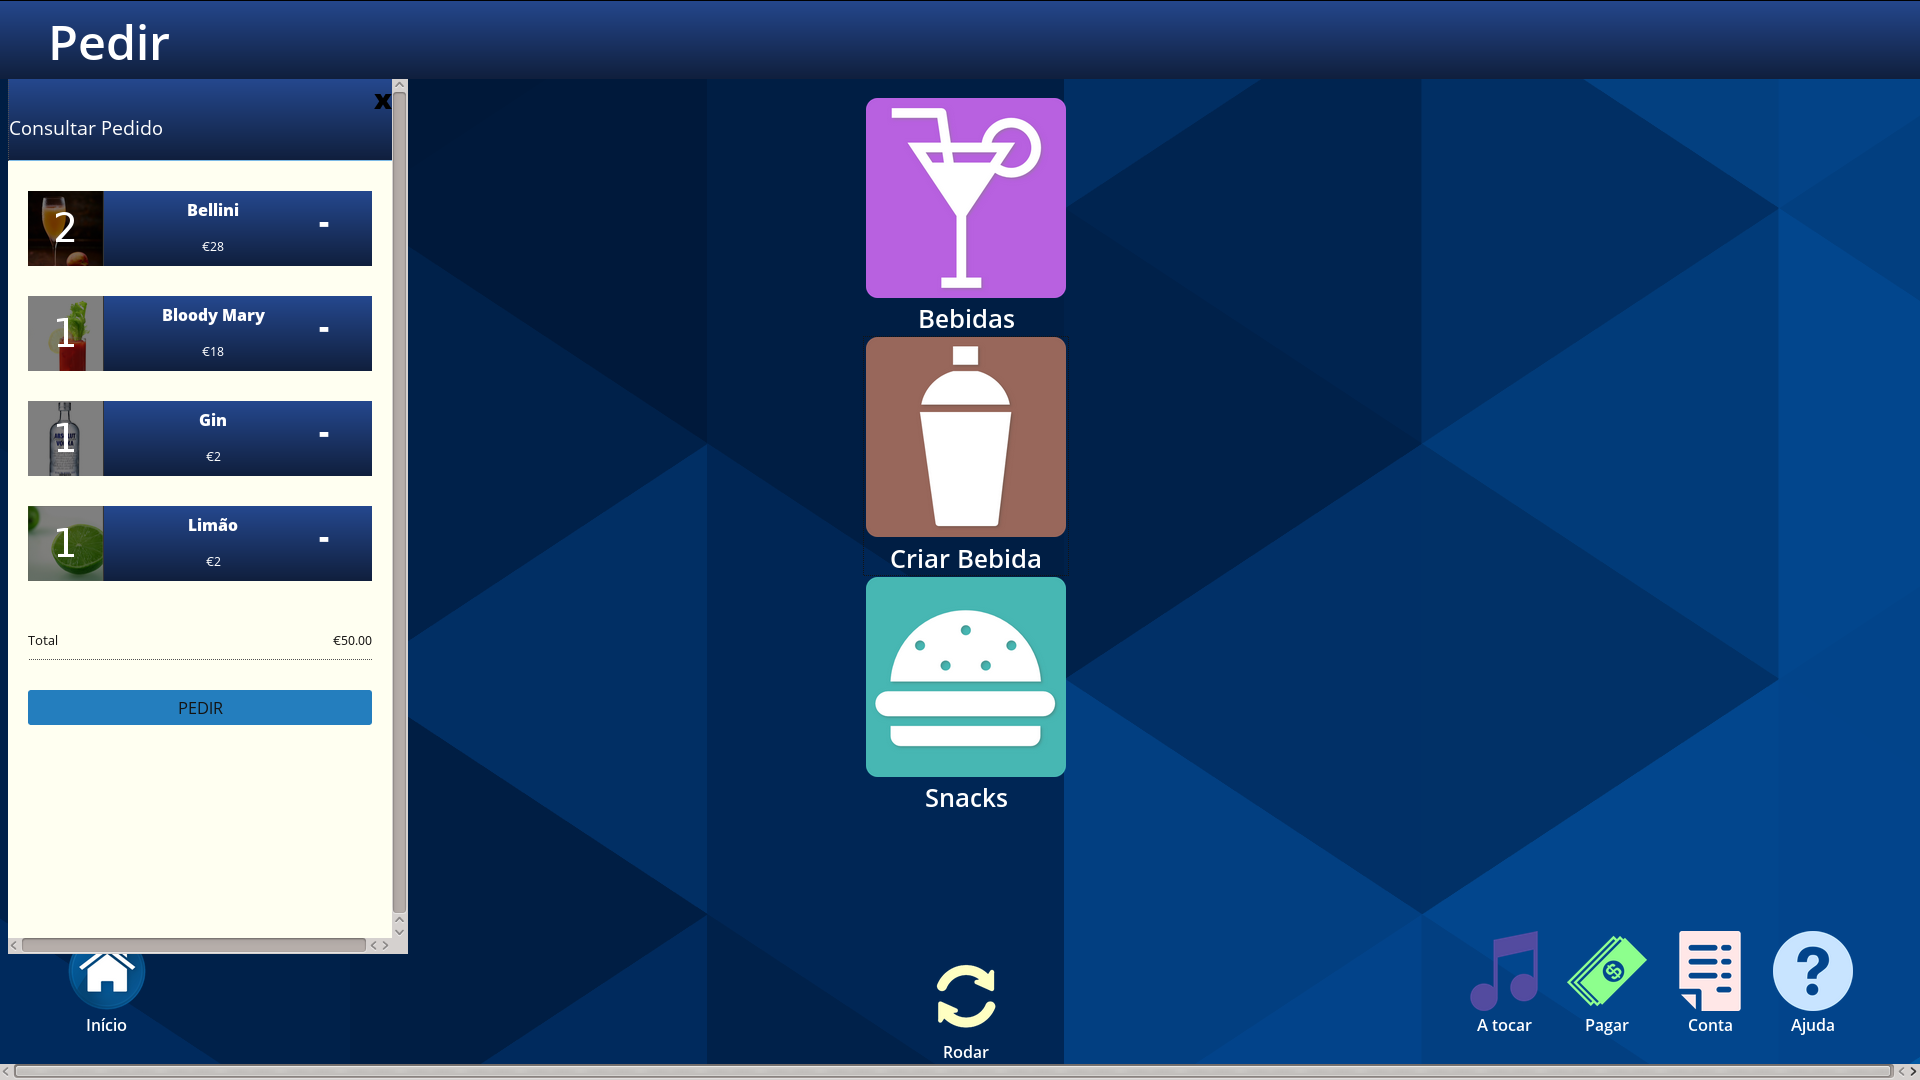
\includegraphics[width=15cm, height=8cm]{user_manual_images/ask_order_submenu.png}
\subsection{Criar uma bebida nova}
\subsection{Pagar}
\subsection{Pedir uma bebida em qualquer ecrã}
\section{Música}
\subsection{Escolher e votar numa música}
\subsection{Ordenar por popularidade}
\subsection{Procurar músicas}
\subsection{Ver atual e próxima música}
\section{Jogos}
\subsection{Escolher um jogo}
\subsection{Eu nunca...}
\subsection{Rolar}
\subsection{Convidar outra mesa}

\end{document}